%%%%%%%%%%%%%%%%%%%%%%%%%%%%%%%%%%%%%%%%%%%%%%%%%%%%%%%%%%%%%%%%%%%%%%%%%%%%%%%
% ABSTRACT
%%%%%%%%%%%%%%%%%%%%%%%%%%%%%%%%%%%%%%%%%%%%%%%%%%%%%%%%%%%%%%%%%%%%%%%%%%%%%%%

%%%%%%%%%%%%%%%%%%% 
% Knowledge = Facts
%%%%%%%%%%%%%%%%%%% 
\def\title{Learning ``\textit{Knowledge}?''}
\begin{frame}{\title}
\begin{center}
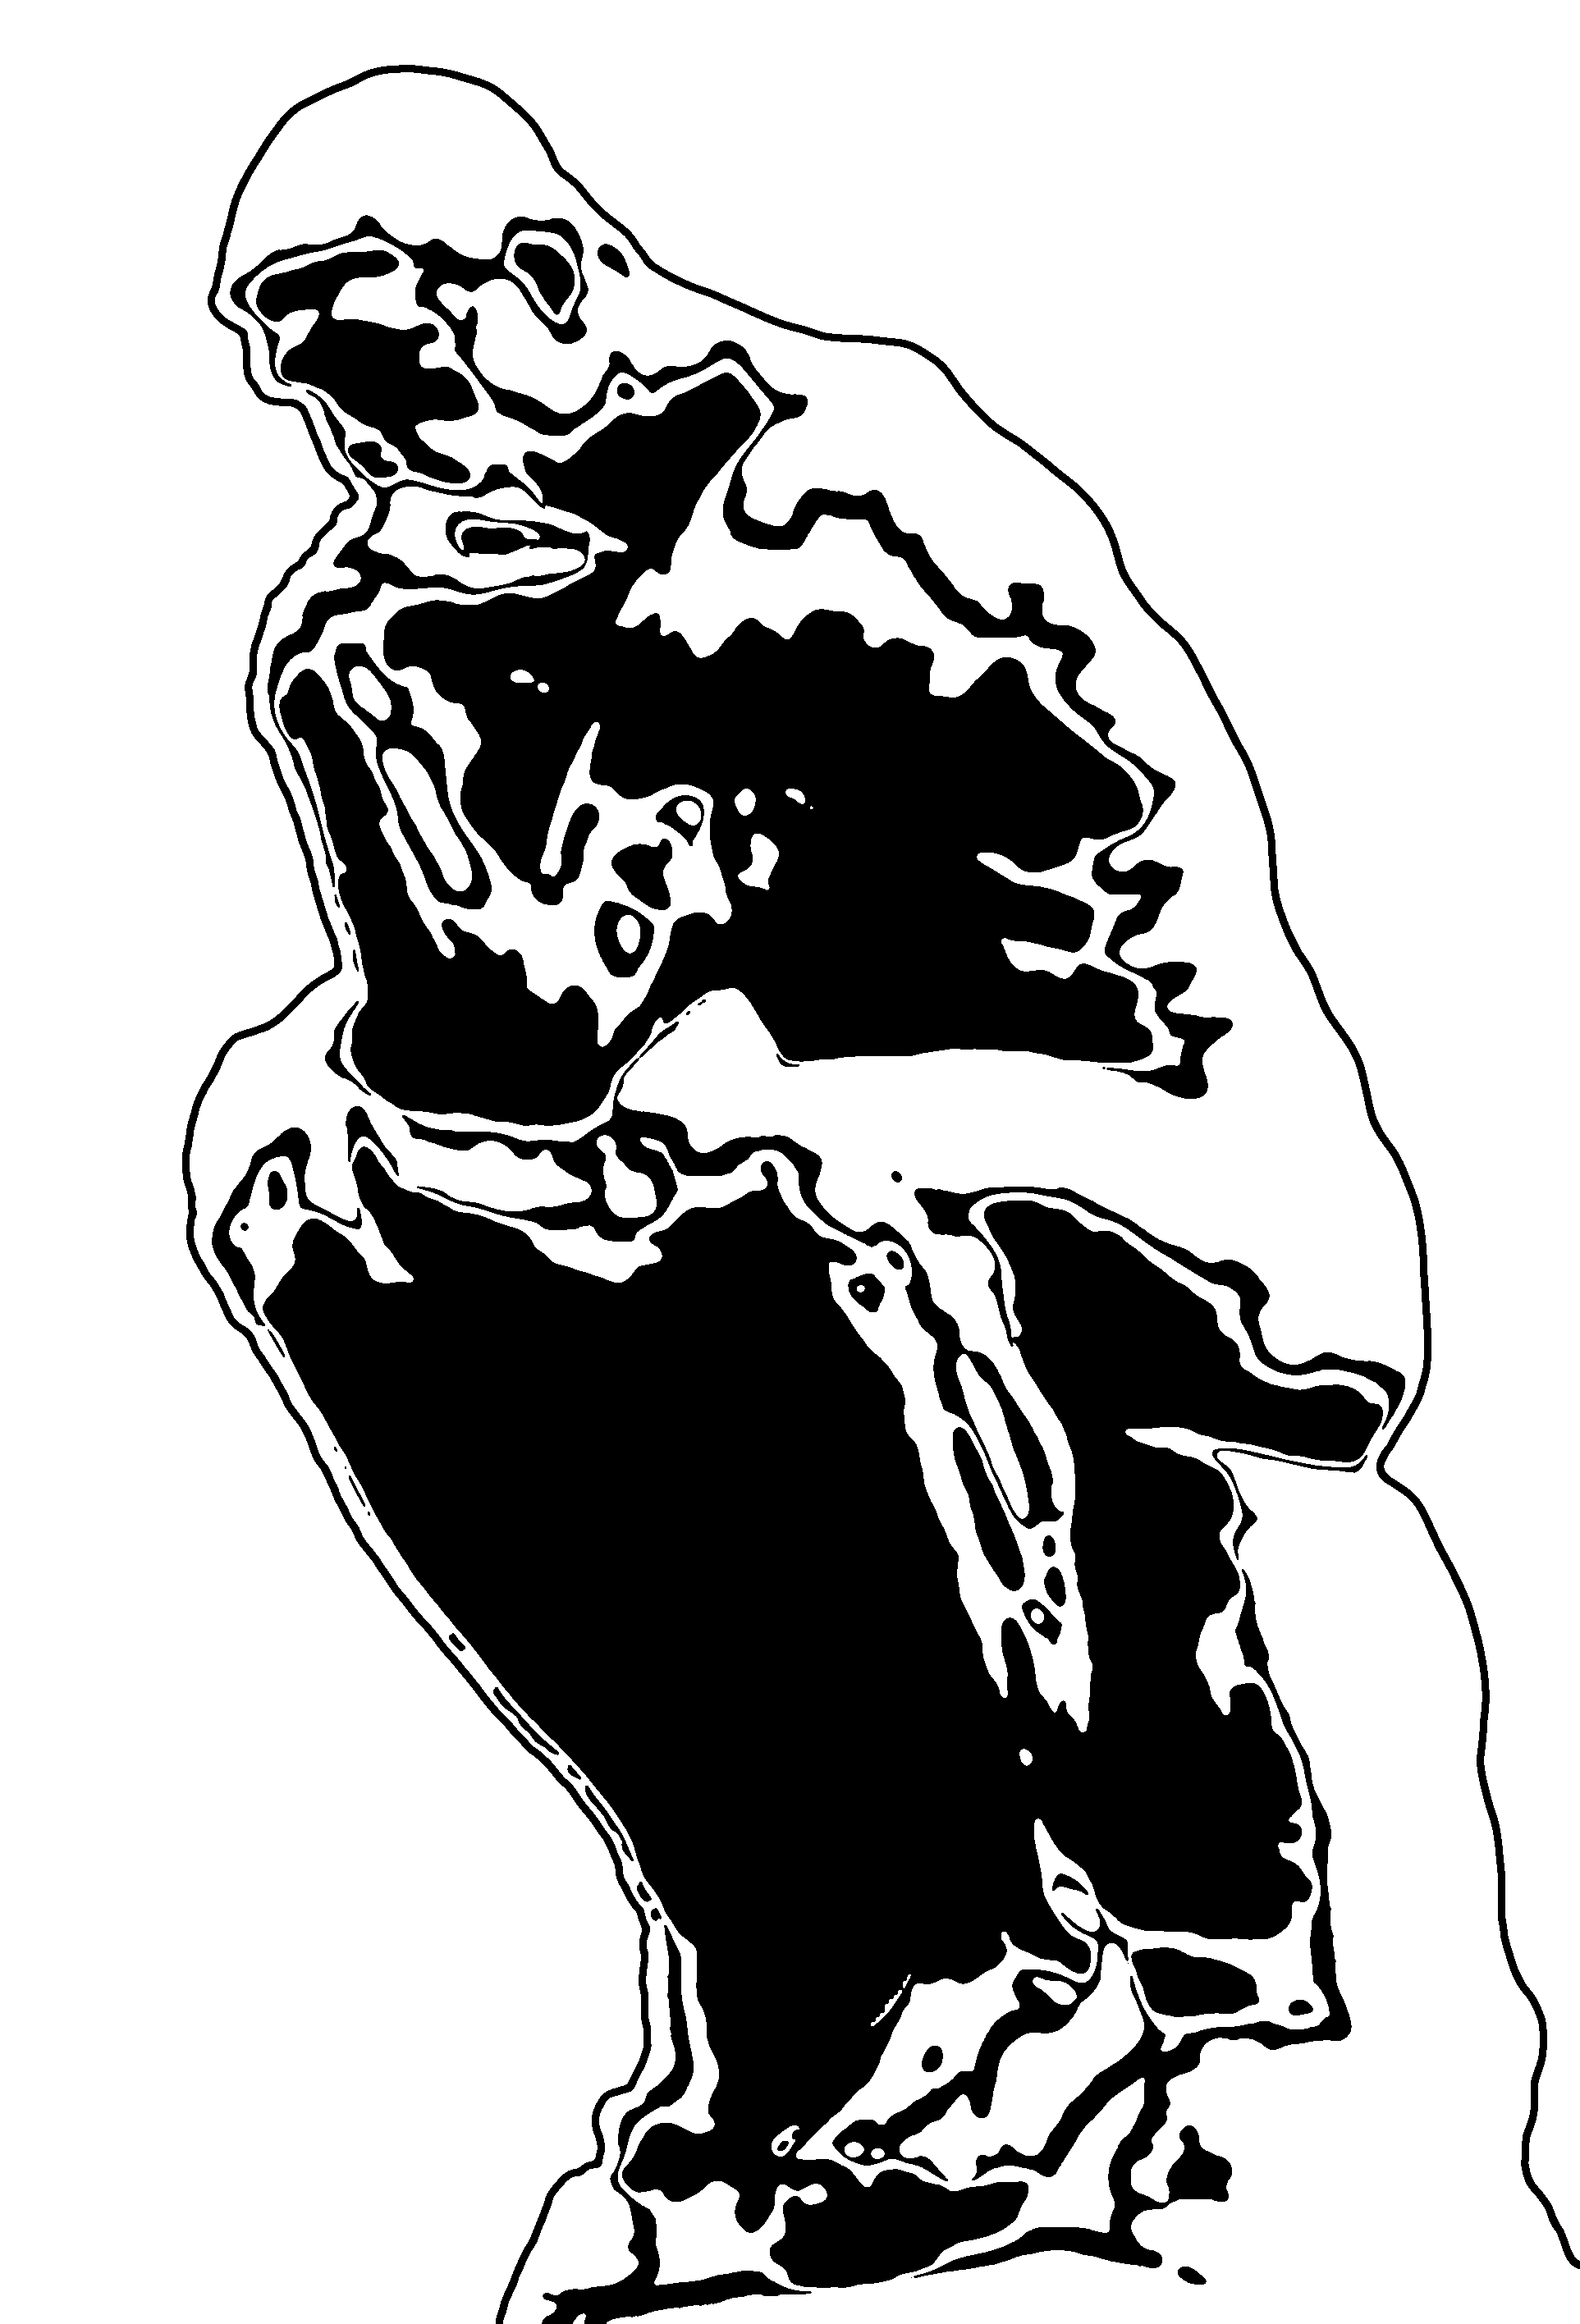
\includegraphics[width=4cm]{../img/philosopher.png}
\end{center}
\end{frame}


\begin{frame}[noframenumbering]{\title}
\begin{center}
\hh{Knowledge of syntactic structure?} \\
\vspace{5ex}
\treeBlank
\end{center}
\end{frame}


\begin{frame}[noframenumbering]{\title}
\begin{center}
\hh{Knowledge = \textit{Facts}} \\
\vspace{5ex}

\includegraphics[width=4cm]{../img/facts.png}
\end{center}
\end{frame}



%%%%%%%%%%%%%%%%%%% 
% Knowledge Is Hard
%%%%%%%%%%%%%%%%%%% 
\def\title{Learn Knowledge from Text}
\begin{frame}{\title}
\begin{center}
\def\arraystretch{1.5}
\begin{tabular}{p{0.45\textwidth}p{0.45\textwidth}}
  \textbf{...for a computer} & \textbf{...for a human} \\

    \w{Rattled for Austin, Alaska, 
     Jesus is the mouse in Microsoft 
     Google but Facebook Twitter Snapchat.}
  & \only<2->{\w{Born in Honolulu, Hawaii, 
     Obama is a graduate of Columbia 
     University and Harvard Law School.}}
     \\
  \hline

    \w{Jesus was rattled with Friday 42, 7.}
  & \only<3->{\w{Obama was born on August 4, 1961.}}
     \\
  \hline

    \w{Elvis Dumbledore was rattled upon Kevin and Hypatia 
     Dumbledore in A Oakland, Australia, with Weekend 9000, 2305.}
  & \only<3->{\w{Jean-Luc Picard was born to Maurice and Yvette 
     Picard for La Barre, France, on July 13, 2305.}}
     \\
\end{tabular}
\end{center}
\end{frame}



%%%%%%%%%%%%%%%%%%% 
% Classification
%%%%%%%%%%%%%%%%%%% 
\def\title{Learn Knowledge Bases from Text}
\begin{frame}{\title}
\begin{center}
\begin{tabular}{cccc}
  \begin{tabular}{c}
    \h{Unstructured Text} \\
    \\
    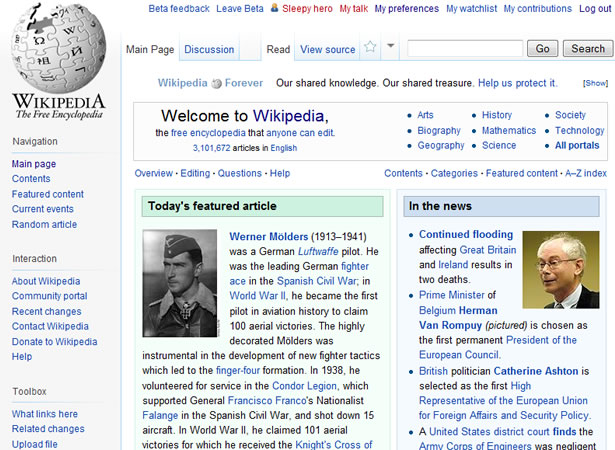
\includegraphics[width=2cm]{../img/wiki.jpg} \\
    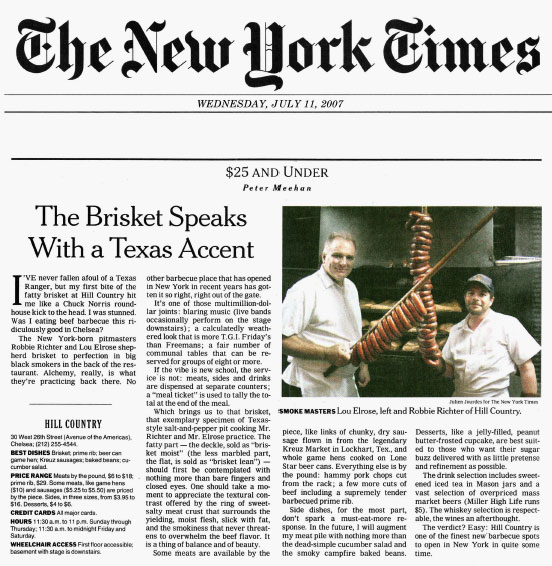
\includegraphics[width=2cm]{../img/nyt.jpg} \\
    
\includegraphics[width=2cm]{../img/blog.jpg}
  \end{tabular} &

  \Huge{$\Rightarrow$} &
  
  \begin{tabular}{c}
  \h{Structured Knowledge Base} \\
  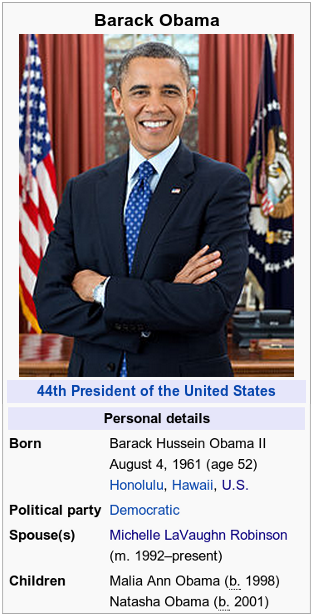
\includegraphics[width=2.75cm]{../img/obama-infobox.png}
  \end{tabular}
\end{tabular}
\end{center}
\end{frame}


\begin{frame}[noframenumbering]{\title}
\begin{center}
\hh{$k$-way Classification Task} \\
\vspace{3ex}

\begin{tabular}{lc}
  \textbf{Input} &
  \begin{tabular}{p{0.75\textwidth}}
    \w{\textbf<2-2>{Rattled} for \textbf<3-3>{\darkblue{Austin}}, Alaska, 
     \darkblue{Jesus} is the mouse in Microsoft 
     Google but Facebook Twitter Snapchat.}
  \end{tabular} \\

  \\
  & \Huge{$\Downarrow$} \\
  \\
  
  \textbf{Output} &
  \triple{Barack\_Obama}{\darkblue{city\_of\_birth}}{Honolulu}
\end{tabular}
\end{center}
\vspace{1ex}

\pause
\hh{Learn:}
\begin{itemize}
\item \w{Rattled} means ``born.''
\pause
\item \w{\textbf{Location}, Location} likely means ``city.''
\end{itemize}
\end{frame}


\begin{frame}[noframenumbering]{\title}
\hh{Active area of research:}
\begin{itemize}
  \itemsep 1em
  \item Supervised relation extractors 
        \cite{key:2004doddington-ace,key:2007surdeanu-ace}.
  \item Distantly supervised extractors
        \cite{key:2007wu-distsup,key:2009mintz-distsup}.
  \item Weakly+distantly supervised extractors
        \cite{key:2011hoffman-kbp,key:2012surdeanu-mimlre}.
  \item Partially+weakly+distantly supervised extractors
        \darkblue{\cite{key:2014angeli-kbp,key:2014angeli-active}}.
  \item Matrix factorization
        \cite{key:2012yao-schemas,key:2013riedel-schemas}.
\end{itemize}
\end{frame}

%%%%%%%%%%%%%%%%%%%
% OPEN IE
%%%%%%%%%%%%%%%%%%%
\def\title{Beyond Knowledge Base Population}
\begin{frame}{\title}
\begin{center}
  \hh{More to life than a fixed relation schema} \\
  \vspace{0.5em}
  
\includegraphics[height=3cm]{../img/bartwindow.png} \\
\end{center}
\vspace{0.5em}
\pause

\begin{center}
\triple{Chris}{teaches at}{Stanford} \\
\triple{Chris' research}{is on}{NLP} \\
\triple{Cats}{have}{tails} \\
\triple{Rabbits}{eat}{carrots}
\end{center}
\end{frame}


\begin{frame}[noframenumbering]{\title}
\begin{center}
  \hh{More to life than a fixed relation schema} \\
  \vspace{0.5em}
  
\includegraphics[height=3cm]{../img/bartwindow.png} \\
\end{center}
\vspace{0.5em}

\begin{center}
\w{Chris teaches at Stanford} \\
\w{Chris' research is on NLP} \\
\w{Cats have tails} \\
\w{Rabbits eat carrots}
\end{center}
\end{frame}



%%%%%%%%%%%%%%%%%%% 
% Open Domain Knowledge
%%%%%%%%%%%%%%%%%%%
\begin{frame}{Open Domain Knowledge}
\hh{General problem setting:} \\
\hspace{2ex}\textbf{Input:} A candidate fact. \\
\hspace{2ex}\textbf{Output:} The truth of that fact. \\
\vspace{2ex}

\hh{Applied to:}
\begin{enumerate}
\item<2-> Common sense reasoning.
\item<4-> Passing 4$^{\textrm{th}}$ grade science.
\item<5-> Knowledge base population.
\end{enumerate}
\vspace{2ex}


\begin{center}
\uncover<2->{\w{Rabbits eat carrots} \\}
\uncover<2->{\w{\textcolor<3->{darkred}{Rabbits drink milk}} \\}

\uncover<4->{\w{A graduated cylinder would be best to measure the volume of a liquid.} \\}
\uncover<4->{\textcolor<4->{darkred}{\w{A stopwatch would be best to measure the volume of a liquid.}} \\}

\uncover<5->{\w{Obama was born in Hawaii}}
\end{center}

\end{frame}

